\documentclass[a4paper, 11pt]{article}
\usepackage[utf8]{inputenc}
\usepackage[left=1in,right=1in,bottom=0.8in]{geometry}
\usepackage{enumitem}
\usepackage{graphicx}
\graphicspath{ {Figures/} }
\usepackage{float}
\usepackage[labelfont=bf]{caption}
\usepackage{fixltx2e}
\usepackage{caption}
\usepackage{amsmath}
\usepackage{capt-of}
\usepackage{minted}
\usepackage{tabu}
\usepackage{pgf}
\usepackage{tikz}
\usetikzlibrary{arrows,automata}

\let\svthefootnote\thefootnote


\title{\bf Experiment 6-7\\\vspace*{2mm} String Recognizer using the Krypton CPLD}
\author{\it Dhruv Ilesh Shah | 150070016}
\date{March 3, 2017}

\begin{document}
\maketitle
\section*{Overview}
Sequential circuits are an important part of digital logic, and hence, in this report, I present the complete implementation of a \emph{string recognizer} that can identify the occurrence of the following words.
\begin{itemize}

	\item bomb
	\item gun
	\item knife
	\item terror
	
\end{itemize}

The code was compiled on Quartus Prime, and simulated using ModelSim. GHDL was also used for simulation purposes, at a low level. This was then uploaded to the {\em Krypton v1.1} 5M1270ZT144C5N CPLD-based board.

The codes and setup have been covered in section 1. We build the string recognizer piece-wise, by implementing each module independently. The VHDL codes have been kept modular and as generic as possible, for reusability and code clarity. Section 2 presents the simulation observations and miscellaneous results. Section 3 presents the observations after running the scan-chain test on the board.

\section{Setup}
The english alphabet can be represented by 5 bits ($\lceil log_2(26) \rceil$), and a bit each for \emph{clock} and \emph{reset} results in 7 input bits. Managing all these, along with keeping track of the states would actually be a tedious task and we would have to deal with a complex machine with close to {\bf 300 states}! That is where the idea of interacting FSMs comes handy. In this report, I implement individual (and independent) FSMs for detecting each of the strings, and an OR of the four outputs gives the required output bit. \par
The inputs were encoding by converting alphabet position (1-26) to 5-bit binary, for simplicity. The various entities used for the detection include \emph{bomber, gunman, knife\_hurler \& terrorist}. The output can be represented with one bit, $1$ standing for positive (string detected!).
\subsection{Bomber}
Straight from the description, a description of the problem in terms of a finite-state machine is given below.
\begin{figure}[h]
\centering

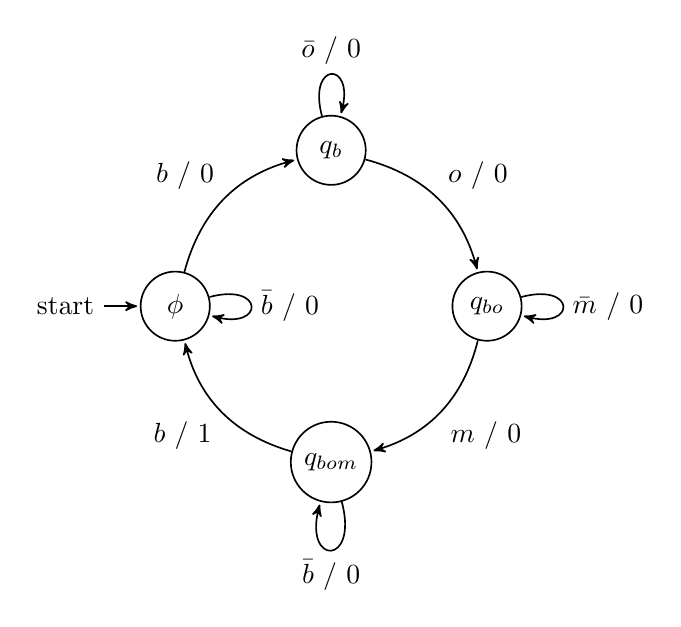
\begin{tikzpicture}[->,>=stealth',shorten >=1pt,auto,node distance=2.8cm,
                    semithick]
  \tikzstyle{every state}=[fill=white,draw=black,text=black]

  \node[initial,state] (A)                    {$\phi$};
  \node[state]         (B) [above right of=A] {$q_b$};
  \node[state]         (D) [below right of=A] {$q_{bom}$};
  \node[state]         (C) [below right of=B] {$q_{bo}$};
%   \node[state]         (E) [below of=D]       {$q_e$};

  \path (A) edge        [bend left]      node {$b$ / 0} (B)
  			edge [loop right] node {$\bar{b}$ / 0} (A)
%             edge              node {1,1,R} (C)
        (B) edge [loop above] node {$\bar{o}$ / 0} (B)
            edge    [bend left]          node {$o$ / 0} (C)
        (C) edge        [bend left]      node {$m$ / 0} (D)
        	edge [loop right] node {$\bar{m}$ / 0} (C)
%             edge [bend left]  node {1,0,R} (E)
        (D) edge [loop below] node {$\bar{b}$ / 0} (D)
            edge [bend left]          node {$b$ / 1} (A);
%         (E) edge [bend left]  node {1,0,R} (A);
\end{tikzpicture}
\caption{Automata Representation for \emph{Bomber}}
\end{figure} \\

As a notation in the above figure, the text on each edge of the graph $a / b$ represents input $a$ to the machine, and output $b$ of the machine. State encoding can be done in a smart way to reduce the combinational overhead for each state bit. For this purpose, I have used \emph{Gray Codes} to encode the states.
\begin{center}
\begin{tabular}{| c | c | c |}
\hline
\bf State & \bf $q_1$ & \bf $q_0$\\
\hline
$\phi$ & 0 & 1 \\
$b$ & 1 & 1 \\
$bo$ &1 & 0 \\
$bom$ & 0 & 0\\
\hline
\end{tabular}
\end{center}
Following the above state assignment and FSM design (Figure 1), the code for detecting \texttt{bomb} is given below.

\inputminted[linenos]{vhdl}{"String Detector/bomb_detector.vhd"}

\subsection{Gunman}

\begin{figure}[H]
\centering

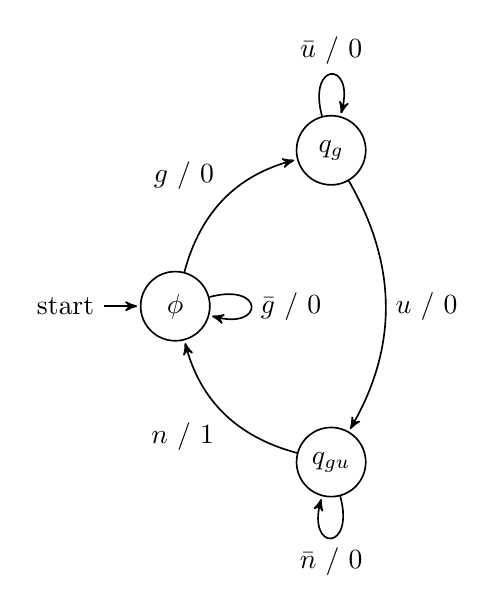
\begin{tikzpicture}[->,>=stealth',shorten >=1pt,auto,node distance=2.8cm,
                    semithick]
  \tikzstyle{every state}=[fill=white,draw=black,text=black]

  \node[initial,state] (A)                    {$\phi$};
  \node[state]         (B) [above right of=A] {$q_g$};
  \node[state]         (D) [below right of=A] {$q_{gu}$};
%   \node[state]         (E) [below of=D]       {$q_e$};

  \path (A) edge        [bend left]      node {$g$ / 0} (B)
  			edge [loop right] node {$\bar{g}$ / 0} (A)
        (B) edge [loop above] node {$\bar{u}$ / 0} (B)
            edge    [bend left]          node {$u$ / 0} (D)
%        (C) edge        [bend left]      node {$m$ / 0} (D)
%        	edge [loop right] node {$\bar{m}$ / 0} (C)
%             edge [bend left]  node {1,0,R} (E)
        (D) edge [loop below] node {$\bar{n}$ / 0} (D)
            edge [bend left]          node {$n$ / 1} (A);
%         (E) edge [bend left]  node {1,0,R} (A);
\end{tikzpicture}
\caption{Automata Representation for \emph{Gunman}}
\end{figure}
Going ahead with the above state representation, the encoding has been done as shown below (since only 2 non-$\phi$ states, one-hot encoding serves the purpose).
\begin{center}
\begin{tabular}{| c | c | c |}
\hline
\bf State & \bf $q_1$ & \bf $q_0$\\
\hline
$\phi$ & 0 & 0 \\
$g$ & 1 & 0 \\
$gu$ &0 & 1 \\
\hline
\end{tabular}
\end{center}
Following the above state assignment and FSM design (Figure 2), the code for detecting \texttt{gun} is given below.
\inputminted[linenos]{vhdl}{"String Detector/gun_detector.vhd"}

\subsection{Knife Hurler}

\begin{figure}[H]
\centering

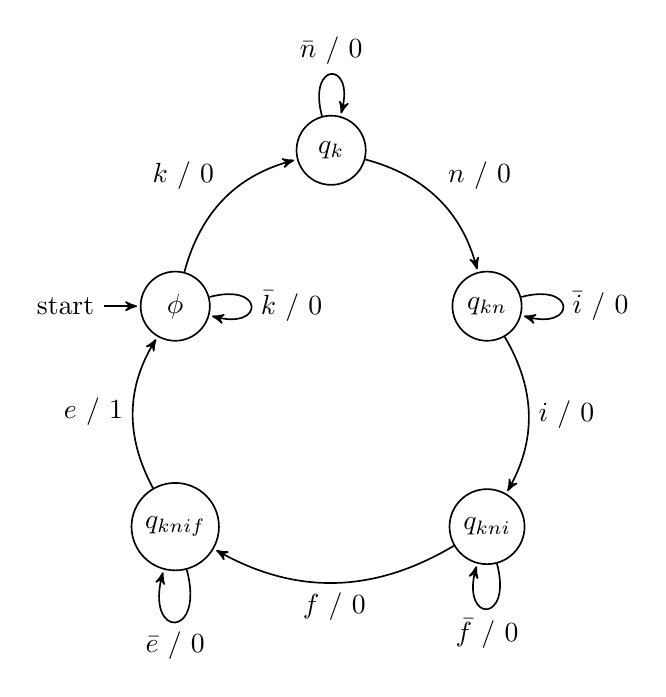
\begin{tikzpicture}[->,>=stealth',shorten >=1pt,auto,node distance=2.8cm,
                    semithick]
  \tikzstyle{every state}=[fill=white,draw=black,text=black]

  \node[initial,state] (A)                    {$\phi$};
  \node[state]         (B) [above right of=A] {$q_k$};
  \node[state]         (D) [below  of=A] {$q_{knif}$};
  \node[state]         (C) [below right of=B] {$q_{kn}$};
   \node[state]         (E) [below of=C]       {$q_{kni}$};

  \path (A) edge        [bend left]      node {$k$ / 0} (B)
  			edge [loop right] node {$\bar{k}$ / 0} (A)
%             edge              node {1,1,R} (C)
        (B) edge [loop above] node {$\bar{n}$ / 0} (B)
            edge    [bend left]          node {$n$ / 0} (C)
        (C) edge        [bend left]      node {$i$ / 0} (E)
        	edge [loop right] node {$\bar{i}$ / 0} (C)
%             edge [bend left]  node {1,0,R} (E)
        (D) edge [loop below] node {$\bar{e}$ / 0} (D)
            edge [bend left]          node {$e$ / 1} (A)
         (E) edge [bend left]  node {$f$ / 0} (D)
         	edge [loop below] node {$\bar{f}$ / 0} (E);
\end{tikzpicture}
\caption{Automata Representation for \emph{Knife Hurler}}
\end{figure}

Going with the above state representation, the encoding requires 3 bits (5 states), and hence I have again followed \emph{Gray Codes} for the encoding. This is shown below.

\begin{center}
\begin{tabular}{| c | c | c | c |}
\hline
\bf State & \bf $q_2$ & \bf $q_1$ & \bf $q_0$\\
\hline
$\phi$ & 0 & 0 & 0 \\
$k$ & 0 & 0 & 1 \\
$kn$  & 0 &1 & 1 \\
$kni$ & 0 & 1 & 0\\
$knif$ & 1 & 1 & 0 \\
\hline
\end{tabular}
\end{center}
Following the above state assignment and FSM design (Figure 3), the code for detecting \texttt{knife} is given below.
\inputminted[linenos]{vhdl}{"String Detector/knife_detector.vhd"}

\subsection{Terrorist}

\begin{figure}[H]
\centering

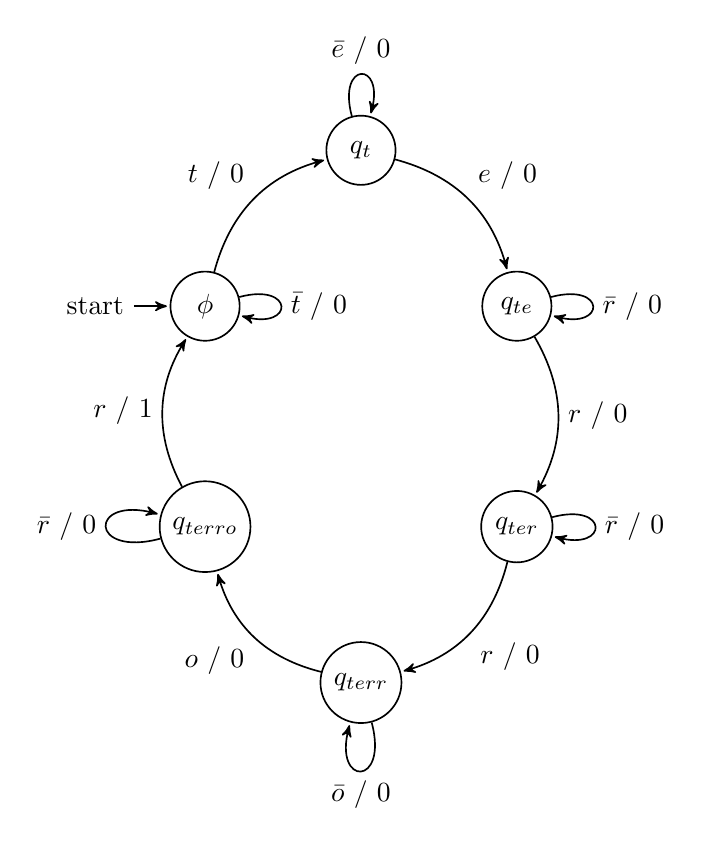
\begin{tikzpicture}[->,>=stealth',shorten >=1pt,auto,node distance=2.8cm,
                    semithick]
  \tikzstyle{every state}=[fill=white,draw=black,text=black]

  \node[initial,state] (A)                    {$\phi$};
  \node[state]         (B) [above right of=A] {$q_t$};
  \node[state]         (D) [below  of=A] {$q_{terro}$};
  \node[state]         (C) [below right of=B] {$q_{te}$};
   \node[state]         (E) [below of=C]       {$q_{ter}$};
   \node [state]			(F) [below left of=E] {$q_{terr}$};

  \path (A) edge        [bend left]      node {$t$ / 0} (B)
  			edge [loop right] node {$\bar{t}$ / 0} (A)
%             edge              node {1,1,R} (C)
        (B) edge [loop above] node {$\bar{e}$ / 0} (B)
            edge    [bend left]          node {$e$ / 0} (C)
        (C) edge        [bend left]      node {$r$ / 0} (E)
        	edge [loop right] node {$\bar{r}$ / 0} (C)
%             edge [bend left]  node {1,0,R} (E)
        (D) edge [loop left] node {$\bar{r}$ / 0} (D)
            edge [bend left]          node {$r$ / 1} (A)
        (F) edge [bend left] node {$o$ / 0} (D)
	        edge [loop below] node {$\bar{o}$ / 0} (F)
         (E) edge [bend left]  node {$r$ / 0} (F)
         	edge [loop right] node {$\bar{r}$ / 0} (E);
\end{tikzpicture}
\caption{Automata Representation for \emph{Terrorist}}
\end{figure}
Going with the above state representation, the encoding requires 3 bits (6 states), and hence I have, yet again, followed \emph{Gray-like Codes} for encoding the states.
\begin{center}
\begin{tabular}{| c | c | c | c |}
\hline
\bf State & \bf $q_2$ & \bf $q_1$ & \bf $q_0$\\
\hline
$\phi$ & 0 & 0 & 0 \\
$t$ & 0 & 0 & 1 \\
$te$  & 0 &1 & 1 \\
$ter$ & 0 & 1 & 0\\
$terr$ & 1 & 1 & 0 \\
$terro$ & 1 & 0 & 0 \\
\hline
\end{tabular}
\end{center}

Following the above state assignment and FSM design (Figure 4), the code for detecting \texttt{terror} is given below.
\inputminted[linenos]{vhdl}{"String Detector/terror_detector.vhd"}

\subsection*{Bringing it all Together}
Now that we have 4 independent FSMs that seem to be doing their job right, we must put them all together, in order to obtain the machine as required in the problem description. Without much effort, this can be done by simply taking an OR operation of the 4 individual outputs. This has been done in the \texttt{DUT}.

\inputminted[linenos]{vhdl}{"String Detector/DUT.vhd"}

\section{Observations}
After implementing the design in code, the next major part is to simulate and test the code for a set of inputs. RTL and Gate-Level simulation was performed on the machine, as a whole. Snapshots of the same are given in Figures 5-8. The validity of the code can be ascertained by the fact that all test cases passed successfully.

\begin{figure}[H]
\centering
\includegraphics[scale=0.33]{RTL}
\caption{RTL Simulation of the String Detector}
\end{figure}

\begin{figure}[H]
\centering
\includegraphics[scale=0.33]{Gate}
\caption{Gate-level Simulation of the String Detector}
\end{figure}

\begin{figure}[H]
\centering
\includegraphics[scale=0.33]{Gate2}
\caption{Gate-level Simulation Zoomed-in to a smaller time frame}
\end{figure}

\section{Scan-Chain Tests}

We have tested the logic using the RTL simulations, emulated the CPLD performance using the gate-level simulation and uploaded the code on the Krypton board. Next, we need to check that the code is actually running as it is expected to, on the board. We could do so manually but that is not feasible due to the following reasons.
\begin{itemize}
	\item Our current circuit requires 7 control switches, including a clock. In any given setup, it \emph{may} not be possible to allocate as many I/O pins. As the complexity increases, it will indeed not be possible to allocate so many pins.
	\item Even if the above is possible, the total number of test cases is \emph{exponential} in the size of the input and it is impractical to perform each of this manually.\footnote{It is not wise to skip any case because, say, we do miss out a failed case it can cascade into unimaginable consequences, which can become difficult to debug.}
\end{itemize}

Hence, we test the uploaded code on the hardware using the scan-chain setup, as suggested in the manual. This setup was run on a set of two collections of text which has occurrences of the concerned string.

\subsection*{Results}
\begin{figure}[H]
\centering
\includegraphics[scale=0.66]{Complete_Test}
\caption{Results of the scan-chain test for random sample test cases.}
\end{figure}


\section*{Conclusion}
Starting from the very scratch, in this report, I have presented the logic and code for a sequential implementation of a string recognizer. The logic was tested using RTL simulation, followed by the gate-level simulation for delay analysis and emulating the CPLD. This was followed by an actual rigorous test on the CPLD board after burning the code on it, using the \emph{TIVA-C} microcontroller.
\par
All the cases passed successfully at all stages and hence the complete string recognizer can be used in hardware, as required.
\end{document}
